\section{有限传播}
\label{sec:wave-finite-speed}

一维公式告诉我们扰动以速度$c$传播。公式本身不能搬到高维，但这个结论能否脱离公式、在任意维成立？答案是能，用的是把能量局部化到一个收缩的球上。

\paragraph{收缩球上的能量}
设$u$在$\mathbb{R}^{d}$上解无源波动方程。取一点$(\bm{x}_0,t_0)$，考虑以$\bm{x}_0$为中心、半径随时间减小的球：
\[
 B_t=B\bigl(\bm{x}_0,\,c(t_0-t)\bigr),\qquad 0\leq t<t_0 .
\]
这些球叠起来就是顶点在$(\bm{x}_0,t_0)$的\term{传播锥}（propagation cone），如图~\ref{fig:wave-cone-proof}：
\begin{equation}
 K=\bigl\{(\bm{x},t):\lVert\bm{x}-\bm{x}_0\rVert_2\leq c(t_0-t),\ 0\leq t\leq t_0\bigr\}.
 \label{eq:wave-cone}
\end{equation}

直观上，球内的能量有两种变化。一是通过球面的能量通量，它可能把能量带进来；二是球在缩小，边缘上的能量被甩到球外。下面的计算说明，后者足以抵消前者，这恰好需要收缩的速度等于波速。

\begin{BookInlineFigure}
  \centering
  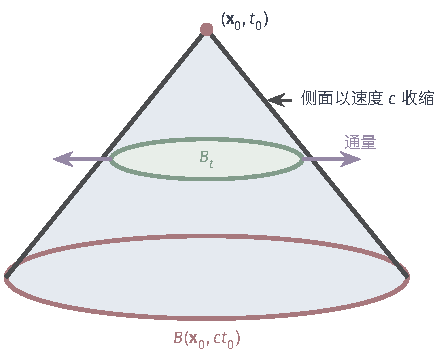
\includegraphics[width=75.406mm]{figures/06-differential-equations/02-partial-differential-equations/tikz/wave-cone-proof/figure.pdf}
  \caption{传播锥。绿色圆盘是时刻$t$的球$B_t$，红色边界是初始的球$B(\bm{x}_0,ct_0)$。紫色箭头是通过球面的能量通量，球的半径以速度$c$减小，通量带来的增量被缩小带走的能量抵消。}
  \label{fig:wave-cone-proof}
\end{BookInlineFigure}

\begin{theorem}[\term{有限传播速度}（finite speed of propagation）]
\label{thm:wave-finite-speed}
设$u\in C^{2}(\mathbb{R}^{d}\times[0,T])$满足$\partial_t^{2}u=c^{2}\Delta u$，$0<t_0\leq T$。若在球$B(\bm{x}_0,ct_0)$上$u_0=u_1=0$，则在传播锥$K$上$u=0$。
\end{theorem}

\begin{proof}
定义局部能量
\[
 e(t)=\frac12\int_{B_t}\bigl[(\partial_tu)^{2}+c^{2}\lVert\nabla u\rVert_2^{2}\bigr]\,\mathrm{d}\bm{x},\qquad 0\leq t<t_0 .
\]
半径变化的球上的积分对$t$求导，除了被积函数的导数，还要加上半径的变化率乘以球面上的积分，这里半径变化率是$-c$。于是
\[
 e'(t)=\int_{B_t}\bigl[\partial_tu\,\partial_t^{2}u+c^{2}\nabla u\cdot\nabla\partial_tu\bigr]\,\mathrm{d}\bm{x}-\frac c2\int_{\partial B_t}\bigl[(\partial_tu)^{2}+c^{2}\lVert\nabla u\rVert_2^{2}\bigr]\,\mathrm{d}S .
\]

和定理~\ref{thm:wave-energy-identity}的证明一样，第一个积分用散度定理和方程化成球面积分，$\bm{n}$为球面的外法向：
\[
 e'(t)=\int_{\partial B_t}\Bigl[c^{2}\partial_tu\,\partial_{\bm{n}}u-\frac c2(\partial_tu)^{2}-\frac{c^{3}}2\lVert\nabla u\rVert_2^{2}\Bigr]\,\mathrm{d}S .
\]

现在估计第一项。法向导数是梯度在单位向量上的分量，所以它的绝对值不超过梯度的范数：
\[
 \lvert\partial_{\bm{n}}u\rvert\leq\lVert\nabla u\rVert_2 .
\]
再对$\lvert\partial_tu\rvert$和$c\lVert\nabla u\rVert_2$用均值不等式：
\[
 c^{2}\lvert\partial_tu\rvert\,\lvert\partial_{\bm{n}}u\rvert\leq c\cdot\lvert\partial_tu\rvert\cdot c\lVert\nabla u\rVert_2\leq\frac c2(\partial_tu)^{2}+\frac{c^{3}}2\lVert\nabla u\rVert_2^{2} .
\]
被积函数因此不超过零，$e'(t)\leq0$。

由假设$e(0)=0$，而$e\geq0$，所以$e(t)=0$对$0\leq t<t_0$成立。于是在$K$内$\partial_tu=0$且$\nabla u=0$。对$K$内任一点$(\bm{x},t)$，线段$\{(\bm{x},s):0\leq s\leq t\}$都在$K$内，沿它积分得$u(\bm{x},t)=u(\bm{x},0)=0$。
\end{proof}

证明中均值不等式的系数恰好是$c/2$，这说明波速$c$是能用的最小收缩速度。球若以更慢的速度收缩，结论就不再成立。取$d=1$，$c=1$，向右传播的帐篷$u=\Lambda(x+5-t)$，支集在$[t-6,t-4]$。$t=0$时支集是$[-6,-4]$，所以$u_0,u_1$在$(-4,4)$上都为零。

让半径按$R(t)=4-t/2$缩小，速度只有$1/2$。这个慢收缩的区间的左端$-R(t)$向右移动得比波包慢，波包追上并进入区间：$t=0$时局部能量为$0$，$t=4$时波包全部在$[-2,0]$内，局部能量等于波包的全部能量$2$。特别地，$u(0,5)=\Lambda(0)=1\neq0$。但这并不违反定理：以$B(0,4)$为底、以速度$1$收缩的锥顶点在$t=4$，点$(0,5)$在锥外。

证明只用到$K$内的方程，所以源项在$K$内为零时结论仍然成立。在有界区域上，只要传播锥不碰到边界，结论就不变；锥碰到固定端或自由端时，边界上的通量项为零，同样的估计在球与$\Omega$的交上仍然有效，端点的影响体现为反射，传播速度依然不超过$c$。

\paragraph{用帐篷核对局部能量}
取$d=1$，$c=1$，帐篷初值，$(x_0,t_0)=(0,3)$，锥在时刻$t$的截面是$\lvert x\rvert\leq3-t$。解$u=F(x-t)+G(x+t)$时，
\[
 (\partial_tu)^{2}+(\partial_xu)^{2}=2F'(x-t)^{2}+2G'(x+t)^{2},
\]
交叉项相消。这里$F=G=\frac12\Lambda$，$\lvert F'\rvert=\frac12$，所以每列波在支集上的能量密度是$\frac12\cdot2\cdot\frac14=\frac14$，长度为$2$，每列带能量$1/2$。

右行波的支集是$[t-1,t+1]$。$t\leq1$时它全在截面内，$e(t)=1$。$t\geq2$时$t-1\geq3-t$，它全部离开截面，$e(t)=0$。$1<t<2$时，留在截面内的长度是$(3-t)-(t-1)=4-2t$，左右两列对称，于是
\begin{equation}
 e(t)=2\cdot\frac14\cdot(4-2t)=2-t,\qquad 1\leq t\leq2.
 \label{eq:wave-local-energy-example}
\end{equation}

这条曲线画在图~\ref{fig:wave-cone-energy}(b)中。局部能量从不增加，波包穿过锥面时能量离开，这正是定理证明中的不等式。(a)是同一过程的时空图。

\begin{BookInlineFigure}
  \centering
  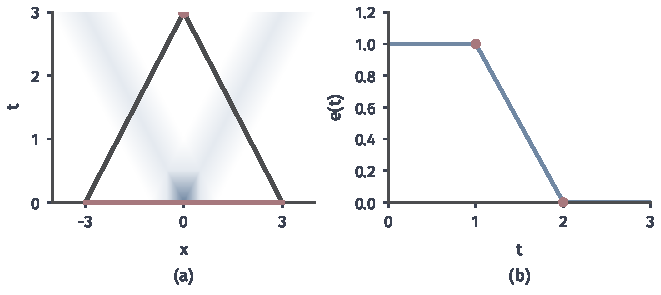
\includegraphics[width=112mm]{figures/06-differential-equations/02-partial-differential-equations/matplotlib/wave-cone-energy/figure.pdf}
  \caption{帐篷解的局部能量，$c=1$，$(x_0,t_0)=(0,3)$。(a)时空图，深灰三角形是传播锥，红色线段是底面。两个波包在$1<t<2$时穿出锥面。(b)由数值积分算出的$e(t)$（蓝），红点标出$t=1,2$，中间一段是式~\eqref{eq:wave-local-energy-example}的直线。}
  \label{fig:wave-cone-energy}
\end{BookInlineFigure}

\paragraph{依赖区域与影响区域}
定理~\ref{thm:wave-finite-speed}可以换一种说法。对线性问题，两个解之差仍是解，所以定理说明：两组初值若在$B(\bm{x}_0,ct_0)$上相同，解在点$(\bm{x}_0,t_0)$的值也相同。这引出下面两个概念。

\begin{definition}[依赖区域与影响区域]
\label{def:wave-domains}
点$(\bm{x}_0,t_0)$的\term{依赖区域}（domain of dependence）是初始时刻的闭球$\overline{B}(\bm{x}_0,ct_0)$。集合$A\subset\mathbb{R}^{d}$的\term{影响区域}（domain of influence）是
\begin{equation}
 \bigl\{(\bm{x},t):t\geq0,\ \mathrm{dist}(\bm{x},A)\leq ct\bigr\}.
 \label{eq:wave-influence}
\end{equation}
\end{definition}

由定理~\ref{thm:wave-finite-speed}，若$u_0,u_1$的支集在$A$内，则$\mathrm{dist}(\bm{x},A)>ct$时$u(\bm{x},t)=0$：以$\bm{x}$为中心、$ct$为半径的球与$A$不相交，初值在球上为零。一维时这两个区域就是图~\ref{fig:wave-dependence}。

定义给出的是“最多”依赖哪些数据，真正依赖的集合可能更小。一维时初始位移只用到两个端点，定理~\ref{thm:wave-finite-speed}无法看出这一点，它只说依赖不会超出球。

\paragraph{与热方程比较}
热方程的解由热核表示。第~\ref{chap:diffusion-equations}章的热核在一维是下面的Gauss函数，$\partial_tu=\partial_x^{2}u$的解是它与初值的卷积：
\[
 \Phi(x,t)=\frac1{\sqrt{4\pi t}}\exp\Bigl(-\frac{x^{2}}{4t}\Bigr),\qquad t>0 .
\]
$\Phi$处处为正，所以非负且不恒为零的初值在任何正时刻都使解处处为正。扰动的“速度”是无穷大的，这和有限传播形成对比。

这个差别需要谨慎理解。取$x=2$，$t=0.01$，单位点源的热核值是
\[
 \Phi(2,0.01)=\frac{\mathrm{e}^{-100}}{\sqrt{0.04\pi}}\approx1.0\times10^{-43},
\]
严格为正，但实际上探测不到。热方程的“无穷速度”是数学结论，物理上是极微弱的尾部。波动方程的前沿外严格为零，不存在尾部。图~\ref{fig:wave-vs-heat-spread}在同一帐篷初值下比较了两者，(c)取对数坐标才看得到热方程的尾部。

\begin{BookInlineFigure}
  \centering
  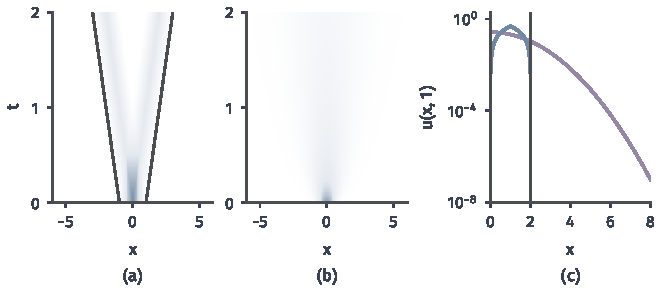
\includegraphics[width=112mm]{figures/06-differential-equations/02-partial-differential-equations/matplotlib/wave-vs-heat-spread/figure.pdf}
  \caption{同一帐篷初值的传播。(a)波动方程（$c=1$）的时空图，深灰线是传播前沿，线外严格为零。(b)热方程（扩散系数为$1$）的时空图，无明确前沿，鼓包逐渐抹平。(c)$t=1$时的对数坐标：紫线是热方程的解，始终为正；蓝线是波动方程的解，到深灰竖线$x=2$处截止。}
  \label{fig:wave-vs-heat-spread}
\end{BookInlineFigure}

\paragraph{耗散与平滑}
除了传播范围，两个方程在耗散和平滑上的差别也来自时间因子。由式~\eqref{eq:wave-pluck-coefficients}，拨弦的第$9$个系数是$a_9=4/(81\pi^{2})\approx0.0050$。$t=0.1$时，$L=1$的两种时间因子分别是
\[
 \mathrm{e}^{-81\pi^{2}\cdot0.1}\approx1.9\times10^{-35},\qquad \cos(0.9\pi)\approx-0.95 .
\]

热方程几乎抹掉了这个模式，波动方程只是改变了它的符号。把所有高频模式放在一起，热方程的解在任意正时刻都是光滑的，波动方程的折角却原样保留，因此逐点的光滑性不可能改善。

反过来，波动方程也没有扩散方程那样的不可逆性。能量不耗散，时间反向后问题仍然适定，高频成分不会在反向时被放大。第~\ref{chap:diffusion-equations}章的逆热问题之所以不稳定，正是因为反向时需要除以极小的因子$\mathrm{e}^{-n^{2}\pi^{2}t}$，而这里的因子模长始终不超过$1$，没有小到需要除的问题。

\paragraph{不要把一维公式搬到高维}
d'Alembert公式依赖换元~\eqref{eq:wave-characteristic-form}，而高维方向不止左右两个，公式没有直接的推广。三维的径向解可以说明这一点。对只依赖$r=\lVert\bm{x}\rVert_2$的函数，$\Delta u=r^{-1}\partial_r^{2}(ru)$，所以$ru$满足一维波动方程。取支集在$(a,b)$内（$a>0$）的光滑函数$\varphi$，外传的球面波是
\begin{equation}
 u(\bm{x},t)=\frac{\varphi(r-ct)}{r} .
 \label{eq:wave-spherical}
\end{equation}
它的幅度按$1/r$衰减，而能量由定理~\ref{thm:wave-energy-identity}（用足够大的球）保持不变：能量摊到越来越大的球面上，每点的振幅自然下降。这比一维行波多了一个衰减因子，是能量守恒与振幅不变并非一回事的另一个例子。

点脉冲的响应在不同维数中的差别更大，如图~\ref{fig:wave-point-response-dimensions}（$c=1$，$t=1$）。一维的响应是$(-1,1)$上的常数$1/2$，前沿过后留下平台。二维的响应在圆盘内是$1/(2\pi\sqrt{1-r^{2}})$，前沿过后留有逐渐衰减的尾巴。三维的响应集中在球面$r=1$上，前沿过后立即归零。这些公式的推导要用到球面平均和降维，篇幅较长，读者可查阅偏微分方程教材。这里要记住的是：前沿之外为零在所有维数中都成立，这是定理~\ref{thm:wave-finite-speed}保证的；前沿之内的形状随维数变化，不能由一维类推。

\begin{BookInlineFigure}
  \centering
  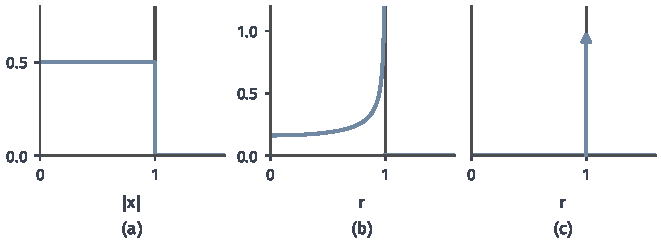
\includegraphics[width=112mm]{figures/06-differential-equations/02-partial-differential-equations/matplotlib/wave-point-response-dimensions/figure.pdf}
  \caption{原点处单位脉冲在$t=1$的响应，$c=1$，横轴为到原点的距离。(a)一维：前沿内是常数$1/2$。(b)二维：前沿内是$1/(2\pi\sqrt{1-r^{2}})$，在$r=1$处发散。(c)三维：全部集中在球面$r=1$上（箭头表示$\delta$分布）。深灰竖线是前沿$r=1$，三种情形在前沿外都为零。}
  \label{fig:wave-point-response-dimensions}
\end{BookInlineFigure}
